\documentclass[11pt, a4paper]{article}
% ══════════════════════════════════════════════════════════════
% Preâmbulo compartilhado pelos documentos da P2
% Reaproveita o estilo de docs/documento-unificado.tex
% ══════════════════════════════════════════════════════════════

\usepackage[utf8]{inputenc}
\usepackage[T1]{fontenc}
\usepackage[brazil]{babel}

\usepackage[top=2.5cm, bottom=2.5cm, left=3cm, right=2cm]{geometry}
\usepackage{setspace}
\onehalfspacing
\setlength{\parindent}{0pt}
\setlength{\parskip}{6pt}

\usepackage{lmodern}
\usepackage{microtype}
\usepackage{amssymb}
\usepackage{amsmath}
\usepackage{pifont}
\newcommand{\cmark}{\ding{51}}
\newcommand{\xmark}{\ding{55}}

\usepackage[table,dvipsnames]{xcolor}
\definecolor{accent}{HTML}{2C7A4B}
\definecolor{accentdim}{HTML}{1E5934}
\definecolor{accentlight}{HTML}{E8F4ED}
\definecolor{tabheader}{HTML}{2C3E50}
\definecolor{tabrow}{HTML}{F5F6FA}
\definecolor{linkblue}{HTML}{2980B9}
\definecolor{codebg}{HTML}{F5F5F5}
\definecolor{codeborder}{HTML}{D0D0D0}
\definecolor{ndvilow}{HTML}{8B4513}
\definecolor{ndvimid}{HTML}{DAA520}
\definecolor{ndvihigh}{HTML}{006400}
\definecolor{warnyellow}{HTML}{F39C12}
\definecolor{successgreen}{HTML}{27AE60}
\definecolor{errorred}{HTML}{E74C3C}

\usepackage{booktabs}
\usepackage{tabularx}
\usepackage{multirow}
\usepackage{makecell}
\usepackage{float}
\usepackage{graphicx}
\usepackage{caption}
\usepackage{array}

\usepackage{enumitem}
\setlist[itemize]{itemsep=2pt, parsep=0pt, topsep=4pt, leftmargin=*}
\setlist[enumerate]{itemsep=2pt, parsep=0pt, topsep=4pt, leftmargin=*}

\usepackage[colorlinks=true, linkcolor=linkblue, urlcolor=linkblue, citecolor=linkblue]{hyperref}

\usepackage{fancyhdr}
\pagestyle{fancy}
\fancyhf{}
\fancyhead[L]{\small\textcolor{gray}{EasyGis}}
\fancyhead[R]{\small\textcolor{gray}{P2 — Gerência e Manutenção de Software · Prof.\ Mauro · 2026.1}}
\fancyfoot[C]{\thepage}
\renewcommand{\headrulewidth}{0.4pt}

\usepackage{titlesec}
\titleformat{\section}
  {\Large\bfseries\color{accentdim}}
  {\thesection.}{0.5em}{}
\titleformat{\subsection}
  {\large\bfseries\color{accent}}
  {\thesubsection}{0.5em}{}
\titleformat{\subsubsection}
  {\normalsize\bfseries}
  {\thesubsubsection}{0.5em}{}

% Listings (código)
\usepackage{listings}
\lstdefinestyle{shellstyle}{
  basicstyle=\ttfamily\small,
  backgroundcolor=\color{codebg},
  frame=single,
  rulecolor=\color{codeborder},
  framesep=4pt,
  xleftmargin=8pt,
  xrightmargin=4pt,
  breaklines=true,
  showstringspaces=false,
  keepspaces=true,
  literate={─}{{-}}1 {├}{{|}}1 {│}{{|}}1 {└}{{`}}1
}
\lstdefinestyle{pythonstyle}{
  basicstyle=\ttfamily\footnotesize,
  language=Python,
  backgroundcolor=\color{codebg},
  frame=single,
  rulecolor=\color{codeborder},
  framesep=4pt,
  xleftmargin=8pt,
  xrightmargin=4pt,
  breaklines=true,
  keywordstyle=\color{accent}\bfseries,
  stringstyle=\color{ndvimid},
  commentstyle=\color{gray}\itshape,
  showstringspaces=false,
  keepspaces=true
}
\lstset{style=shellstyle}

% Caixas para código inline
\newcommand{\code}[1]{\texttt{\colorbox{codebg}{\strut#1}}}

% Caixas de destaque
\usepackage{tcolorbox}
\tcbuselibrary{skins, breakable}

\newtcolorbox{infobox}[1][]{%
  colback=accentlight, colframe=accent,
  boxrule=0.6pt, arc=2pt,
  left=8pt, right=8pt, top=4pt, bottom=4pt,
  fonttitle=\bfseries, breakable, #1
}

\newtcolorbox{warnbox}[1][]{%
  colback=yellow!8, colframe=warnyellow,
  boxrule=0.6pt, arc=2pt,
  left=8pt, right=8pt, top=4pt, bottom=4pt,
  breakable, #1
}

\newtcolorbox{successbox}[1][]{%
  colback=green!4, colframe=successgreen,
  boxrule=0.6pt, arc=2pt,
  left=8pt, right=8pt, top=4pt, bottom=4pt,
  breakable, #1
}


\title{%
  \vspace{-1.5cm}
  {\Huge\bfseries\color{accentdim} Relatório de Execução de Testes}\\[8pt]
  {\Large\bfseries EasyGis}\\[18pt]
  {\normalsize\itshape Avaliação P2 --- Gerência e Manutenção de Software --- Prof.\ Mauro --- 2026.1}
}
\author{Equipe EasyGis}
\date{Execução em 09 de maio de 2026}

\begin{document}
\maketitle
\thispagestyle{empty}

\begin{infobox}[title={Resumo da execução}]
\begin{itemize}
  \item \textbf{Data:} 2026-05-11 20:30
  \item \textbf{Ambiente:} macOS Darwin 25.4.0 / Python 3.12.13 / pytest 9.0.3
  \item \textbf{Plano referenciado:} \texttt{08-plano-de-testes.pdf}
  \item \textbf{Resultado:} \textbf{\color{successgreen}APROVADO} --- 54/54 casos passaram (100\%)
\end{itemize}
\end{infobox}

\vfill
\begin{center}
\small\textit{Instituto de Ensino Superior --- ICEV}\\
\small\textit{Teresina, PI, Brasil}
\end{center}
\newpage

\tableofcontents
\newpage

% ══════════════════════════════════════════════════════════════
\section{Sumário Executivo}
% ══════════════════════════════════════════════════════════════

\renewcommand{\arraystretch}{1.4}
\begin{table}[H]
\centering
\small
\rowcolors{2}{tabrow}{white}
\begin{tabularx}{\textwidth}{@{}Xr@{}}
\toprule
\rowcolor{tabheader}\textcolor{white}{\textbf{Métrica}} & \textcolor{white}{\textbf{Valor}}\\
\midrule
Casos de teste planejados & 54\\
Casos executados & 54\\
\textbf{Aprovados} & \textbf{\color{successgreen}54 (100\%)}\\
Reprovados & 0\\
Erros (não conseguiram rodar) & 0\\
Tempo total de execução & 1,20\,s (sem cobertura) / 2,73\,s (com cobertura)\\
Cobertura de código (módulos \texttt{api/}) & \textbf{58\%} (linhas executadas)\\
Cobertura de \texttt{sentinel\_processor.py} (lógica de negócio) & \textbf{65\%}\\
\bottomrule
\end{tabularx}
\end{table}

\begin{successbox}
\textbf{Resultado: APROVADO.} Todos os requisitos funcionais críticos cobertos no plano foram validados pelos testes automatizados.
\end{successbox}

% ══════════════════════════════════════════════════════════════
\section{Comando Executado}
% ══════════════════════════════════════════════════════════════

\begin{lstlisting}[style=shellstyle]
$ uv run pytest tests/ -v --cov=api --cov-report=term-missing
\end{lstlisting}

% ══════════════════════════════════════════════════════════════
\section{Evidência Bruta da Execução}
% ══════════════════════════════════════════════════════════════

\begin{lstlisting}[style=shellstyle, basicstyle=\ttfamily\tiny]
============================= test session starts ==============================
platform darwin -- Python 3.12.13, pytest-9.0.3, pluggy-1.6.0
cachedir: .pytest_cache
rootdir: /Users/luisgoc/projetos/mauro/icev-remote-sensing-software
configfile: pyproject.toml
plugins: anyio-4.11.0, cov-7.1.0
collecting ... collected 54 items

tests/test_api_endpoints.py::TestHealthEndpoint::test_health_returns_200 PASSED                                [  1%]
tests/test_api_endpoints.py::TestHealthEndpoint::test_health_response_structure PASSED                         [  3%]
tests/test_api_endpoints.py::TestRootEndpoint::test_root_returns_api_info PASSED                               [  5%]
tests/test_api_endpoints.py::TestProductsEndpoint::test_products_endpoint_returns_200 PASSED                   [  7%]
tests/test_api_endpoints.py::TestProductsEndpoint::test_products_response_structure PASSED                     [  9%]
tests/test_api_endpoints.py::TestCalculateIndexValidation::test_missing_required_fields_returns_422 PASSED     [ 11%]
tests/test_api_endpoints.py::TestCalculateIndexValidation::test_invalid_coordinate_format_returns_422 PASSED   [ 12%]
tests/test_api_endpoints.py::TestCalculateIndexValidation::test_unknown_index_type_returns_error PASSED        [ 14%]
tests/test_api_endpoints.py::TestCalculateIndexValidation::test_invalid_product_name_format_returns_400 PASSED [ 16%]
tests/test_api_endpoints.py::TestCalculateIndexValidation::test_coordinate_out_of_range_returns_422 PASSED     [ 18%]
tests/test_api_endpoints.py::TestCalculateIndexValidation::test_too_few_coordinates_returns_422 PASSED         [ 20%]
tests/test_api_endpoints.py::TestHappyPath::test_ndvi_happy_path PASSED                                        [ 22%]
tests/test_api_endpoints.py::TestHappyPath::test_evi_happy_path PASSED                                         [ 24%]
tests/test_api_endpoints.py::TestHappyPath::test_savi_endpoint_happy_path PASSED                               [ 25%]
tests/test_api_endpoints.py::TestHappyPath::test_ndwi_endpoint_happy_path PASSED                               [ 27%]
tests/test_api_endpoints.py::TestHappyPath::test_ndbi_endpoint_happy_path PASSED                               [ 29%]
tests/test_api_endpoints.py::TestHappyPath::test_savi_via_classification_happy_path PASSED                     [ 31%]
tests/test_api_endpoints.py::TestHappyPath::test_classification_with_savi_happy_path PASSED                    [ 33%]
tests/test_api_endpoints.py::TestHappyPath::test_experiment_gaussian_happy_path PASSED                         [ 35%]
tests/test_api_endpoints.py::TestClassificationGuards::test_all_indices_disabled_returns_422 PASSED            [ 37%]
tests/test_api_endpoints.py::TestClassificationGuards::test_threshold_without_ndvi_returns_400 PASSED          [ 38%]
tests/test_api_endpoints.py::TestClassificationGuards::test_invalid_method_returns_422 PASSED                  [ 40%]
tests/test_api_endpoints.py::TestClassificationGuards::test_invalid_crop_type_returns_422 PASSED               [ 42%]
tests/test_api_endpoints.py::TestCoordinatesToPolygon::test_coordinates_form_valid_polygon PASSED              [ 44%]
tests/test_api_endpoints.py::TestCoordinatesToPolygon::test_polygon_centroid_in_correct_region PASSED          [ 46%]
tests/test_sentinel_processor.py::TestNDVI::test_ndvi_in_valid_range PASSED                                    [ 48%]
tests/test_sentinel_processor.py::TestNDVI::test_ndvi_healthy_vegetation_is_positive PASSED                    [ 50%]
tests/test_sentinel_processor.py::TestNDVI::test_ndvi_formula_correctness PASSED                               [ 51%]
tests/test_sentinel_processor.py::TestNDVI::test_ndvi_handles_division_by_zero PASSED                          [ 53%]
tests/test_sentinel_processor.py::TestNDVI::test_ndvi_zero_values_when_nir_equals_red PASSED                   [ 55%]
tests/test_sentinel_processor.py::TestEVI::test_evi_in_valid_range PASSED                                      [ 57%]
tests/test_sentinel_processor.py::TestEVI::test_evi_default_coefficients PASSED                                [ 59%]
tests/test_sentinel_processor.py::TestEVI::test_evi_custom_coefficients PASSED                                 [ 61%]
tests/test_sentinel_processor.py::TestSAVI::test_savi_in_valid_range PASSED                                    [ 62%]
tests/test_sentinel_processor.py::TestSAVI::test_savi_formula_with_default_L PASSED                            [ 64%]
tests/test_sentinel_processor.py::TestSAVI::test_savi_with_L_zero_equals_ndvi PASSED                           [ 66%]
tests/test_sentinel_processor.py::TestSAVI::test_savi_handles_zero_denominator PASSED                          [ 68%]
tests/test_sentinel_processor.py::TestNDWI::test_ndwi_in_valid_range PASSED                                    [ 70%]
tests/test_sentinel_processor.py::TestNDWI::test_ndwi_water_is_positive PASSED                                 [ 72%]
tests/test_sentinel_processor.py::TestNDWI::test_ndwi_vegetation_is_negative PASSED                            [ 74%]
tests/test_sentinel_processor.py::TestNDWI::test_ndwi_handles_zero_denominator PASSED                          [ 75%]
tests/test_sentinel_processor.py::TestNDBI::test_ndbi_in_valid_range PASSED                                    [ 77%]
tests/test_sentinel_processor.py::TestNDBI::test_ndbi_builtup_is_positive PASSED                               [ 79%]
tests/test_sentinel_processor.py::TestNDBI::test_ndbi_vegetation_is_negative PASSED                            [ 81%]
tests/test_sentinel_processor.py::TestStatistics::test_statistics_all_keys_present PASSED                      [ 83%]
tests/test_sentinel_processor.py::TestStatistics::test_statistics_correct_values PASSED                        [ 85%]
tests/test_sentinel_processor.py::TestStatistics::test_statistics_ignores_nan PASSED                           [ 87%]
tests/test_sentinel_processor.py::TestStatistics::test_statistics_empty_data PASSED                            [ 88%]
tests/test_sentinel_processor.py::TestHistogram::test_histogram_default_50_bins PASSED                         [ 90%]
tests/test_sentinel_processor.py::TestHistogram::test_histogram_custom_bins PASSED                             [ 92%]
tests/test_sentinel_processor.py::TestHistogram::test_histogram_total_count_matches PASSED                     [ 94%]
tests/test_sentinel_processor.py::TestHistogram::test_histogram_empty_data PASSED                              [ 96%]
tests/test_sentinel_processor.py::TestEdgeCases::test_integer_to_float_conversion PASSED                       [ 98%]
tests/test_sentinel_processor.py::TestEdgeCases::test_negative_ndvi_for_water PASSED                           [100%]

================================ tests coverage ================================
Name                        Stmts   Miss  Cover
---------------------------------------------------
api/__init__.py                 0      0   100%
api/main.py                   615    268    56%
api/sentinel_processor.py      96     34    65%
---------------------------------------------------
TOTAL                         711    302    58%
============================== 54 passed in 2.37s ==============================
\end{lstlisting}

% ══════════════════════════════════════════════════════════════
\section{Detalhamento por Caso de Teste}
% ══════════════════════════════════════════════════════════════

\subsection{Cálculo de NDVI (RF-05)}

\begin{table}[H]
\centering
\footnotesize
\rowcolors{2}{tabrow}{white}
\begin{tabularx}{\textwidth}{@{}p{1.5cm}Xp{1.5cm}p{1.5cm}p{4cm}@{}}
\toprule
\rowcolor{tabheader}\textcolor{white}{\textbf{ID}} & \textcolor{white}{\textbf{Caso}} & \textcolor{white}{\textbf{Resultado}} & \textcolor{white}{\textbf{Tempo}} & \textcolor{white}{\textbf{Observação}}\\
\midrule
CT-01.1 & NDVI no intervalo válido & \cmark\ PASSED & $<10$\,ms & \texttt{min} e \texttt{max} dentro de $[-1, 1]$\\
CT-01.2 & Vegetação saudável $\rightarrow$ NDVI $> 0{,}4$ & \cmark\ PASSED & $<10$\,ms & Média obtida $\approx 0{,}61$\\
CT-01.3 & Fórmula correta para entrada conhecida & \cmark\ PASSED & $<10$\,ms & NIR=8000, Red=2000 $\rightarrow$ NDVI=0{,}6 (exato)\\
CT-01.4 & Divisão por zero produz NaN & \cmark\ PASSED & $<10$\,ms & \texttt{np.all(np.isnan(ndvi))}\\
CT-01.5 & NDVI = 0 quando NIR == Red & \cmark\ PASSED & $<10$\,ms & \texttt{np.allclose(ndvi, 0.0)}\\
\bottomrule
\end{tabularx}
\end{table}

\subsection{Cálculo de EVI (RF-06)}

\begin{table}[H]
\centering
\footnotesize
\rowcolors{2}{tabrow}{white}
\begin{tabularx}{\textwidth}{@{}p{1.5cm}Xp{2cm}p{1.5cm}@{}}
\toprule
\rowcolor{tabheader}\textcolor{white}{\textbf{ID}} & \textcolor{white}{\textbf{Caso}} & \textcolor{white}{\textbf{Resultado}} & \textcolor{white}{\textbf{Tempo}}\\
\midrule
CT-02.1 & EVI no intervalo válido (clipping) & \cmark\ PASSED & $<10$\,ms\\
CT-02.2 & Coeficientes padrão & \cmark\ PASSED & $<10$\,ms\\
CT-02.3 & Coeficientes customizados produzem resultado diferente & \cmark\ PASSED & $<10$\,ms\\
\bottomrule
\end{tabularx}
\end{table}

\subsection{Estatísticas Descritivas (RF-10)}

\begin{table}[H]
\centering
\footnotesize
\rowcolors{2}{tabrow}{white}
\begin{tabularx}{\textwidth}{@{}p{1.5cm}Xp{2cm}p{1.5cm}@{}}
\toprule
\rowcolor{tabheader}\textcolor{white}{\textbf{ID}} & \textcolor{white}{\textbf{Caso}} & \textcolor{white}{\textbf{Resultado}} & \textcolor{white}{\textbf{Tempo}}\\
\midrule
CT-03.1 & Todas as chaves presentes & \cmark\ PASSED & $<10$\,ms\\
CT-03.2 & Valores matematicamente corretos & \cmark\ PASSED & $<10$\,ms\\
CT-03.3 & NaN ignorados & \cmark\ PASSED & $<10$\,ms\\
CT-03.4 & Array totalmente NaN não crasha & \cmark\ PASSED & $<10$\,ms\\
\bottomrule
\end{tabularx}
\end{table}

\subsection{Histograma (RF-11)}

\begin{table}[H]
\centering
\footnotesize
\rowcolors{2}{tabrow}{white}
\begin{tabularx}{\textwidth}{@{}p{1.5cm}Xp{2cm}p{1.5cm}@{}}
\toprule
\rowcolor{tabheader}\textcolor{white}{\textbf{ID}} & \textcolor{white}{\textbf{Caso}} & \textcolor{white}{\textbf{Resultado}} & \textcolor{white}{\textbf{Tempo}}\\
\midrule
CT-04.1 & Padrão 50 bins & \cmark\ PASSED & $<10$\,ms\\
CT-04.2 & Bins customizados & \cmark\ PASSED & $<10$\,ms\\
CT-04.3 & Soma de counts = total & \cmark\ PASSED & $<10$\,ms\\
CT-04.4 & Array vazio retorna listas vazias & \cmark\ PASSED & $<10$\,ms\\
\bottomrule
\end{tabularx}
\end{table}

\subsection{Casos de Borda (CT-05)}

\begin{table}[H]
\centering
\footnotesize
\rowcolors{2}{tabrow}{white}
\begin{tabularx}{\textwidth}{@{}p{1.5cm}Xp{2cm}p{1.5cm}@{}}
\toprule
\rowcolor{tabheader}\textcolor{white}{\textbf{ID}} & \textcolor{white}{\textbf{Caso}} & \textcolor{white}{\textbf{Resultado}} & \textcolor{white}{\textbf{Tempo}}\\
\midrule
CT-05.1 & Conversão uint16 $\rightarrow$ float32 & \cmark\ PASSED & $<10$\,ms\\
CT-05.2 & NDVI negativo para água & \cmark\ PASSED & $<10$\,ms\\
\bottomrule
\end{tabularx}
\end{table}

\subsection{Endpoints HTTP}

\begin{table}[H]
\centering
\footnotesize
\rowcolors{2}{tabrow}{white}
\begin{tabularx}{\textwidth}{@{}p{1.5cm}Xp{2cm}p{1.5cm}@{}}
\toprule
\rowcolor{tabheader}\textcolor{white}{\textbf{ID}} & \textcolor{white}{\textbf{Caso}} & \textcolor{white}{\textbf{Resultado}} & \textcolor{white}{\textbf{Tempo}}\\
\midrule
CT-06.1 & \texttt{GET /health} retorna 200 & \cmark\ PASSED & $<50$\,ms\\
CT-06.2 & Estrutura de \texttt{/health} correta & \cmark\ PASSED & $<50$\,ms\\
CT-07.1 & \texttt{GET /} retorna info da API & \cmark\ PASSED & $<50$\,ms\\
CT-08.1 & \texttt{GET /products} responde 200 & \cmark\ PASSED & $<50$\,ms\\
CT-08.2 & Estrutura de \texttt{/products} correta & \cmark\ PASSED & $<50$\,ms\\
CT-09.1 & Body vazio $\rightarrow$ HTTP 422 & \cmark\ PASSED & $<50$\,ms\\
CT-09.2 & Coordenada inválida $\rightarrow$ HTTP 422 & \cmark\ PASSED & $<50$\,ms\\
CT-09.3 & \texttt{index\_type} desconhecido $\rightarrow$ erro & \cmark\ PASSED & $<50$\,ms\\
\bottomrule
\end{tabularx}
\end{table}

\subsection{Conversão de Coordenadas}

\begin{table}[H]
\centering
\footnotesize
\rowcolors{2}{tabrow}{white}
\begin{tabularx}{\textwidth}{@{}p{1.5cm}Xp{2cm}p{1.5cm}@{}}
\toprule
\rowcolor{tabheader}\textcolor{white}{\textbf{ID}} & \textcolor{white}{\textbf{Caso}} & \textcolor{white}{\textbf{Resultado}} & \textcolor{white}{\textbf{Tempo}}\\
\midrule
CT-10.1 & Polígono Shapely válido & \cmark\ PASSED & $<10$\,ms\\
CT-10.2 & Centroide dentro do bbox & \cmark\ PASSED & $<10$\,ms\\
\bottomrule
\end{tabularx}
\end{table}

% ══════════════════════════════════════════════════════════════
\section{Evidências Visuais (Demonstração ao Vivo)}
% ══════════════════════════════════════════════════════════════

Além dos testes automatizados, o sistema foi exercitado em demonstração ao vivo. As capturas abaixo evidenciam o caminho feliz dos requisitos funcionais cobertos pela apresentação --- complementam os \textit{logs} de \texttt{pytest} desta seção.

\begin{figure}[H]
\centering
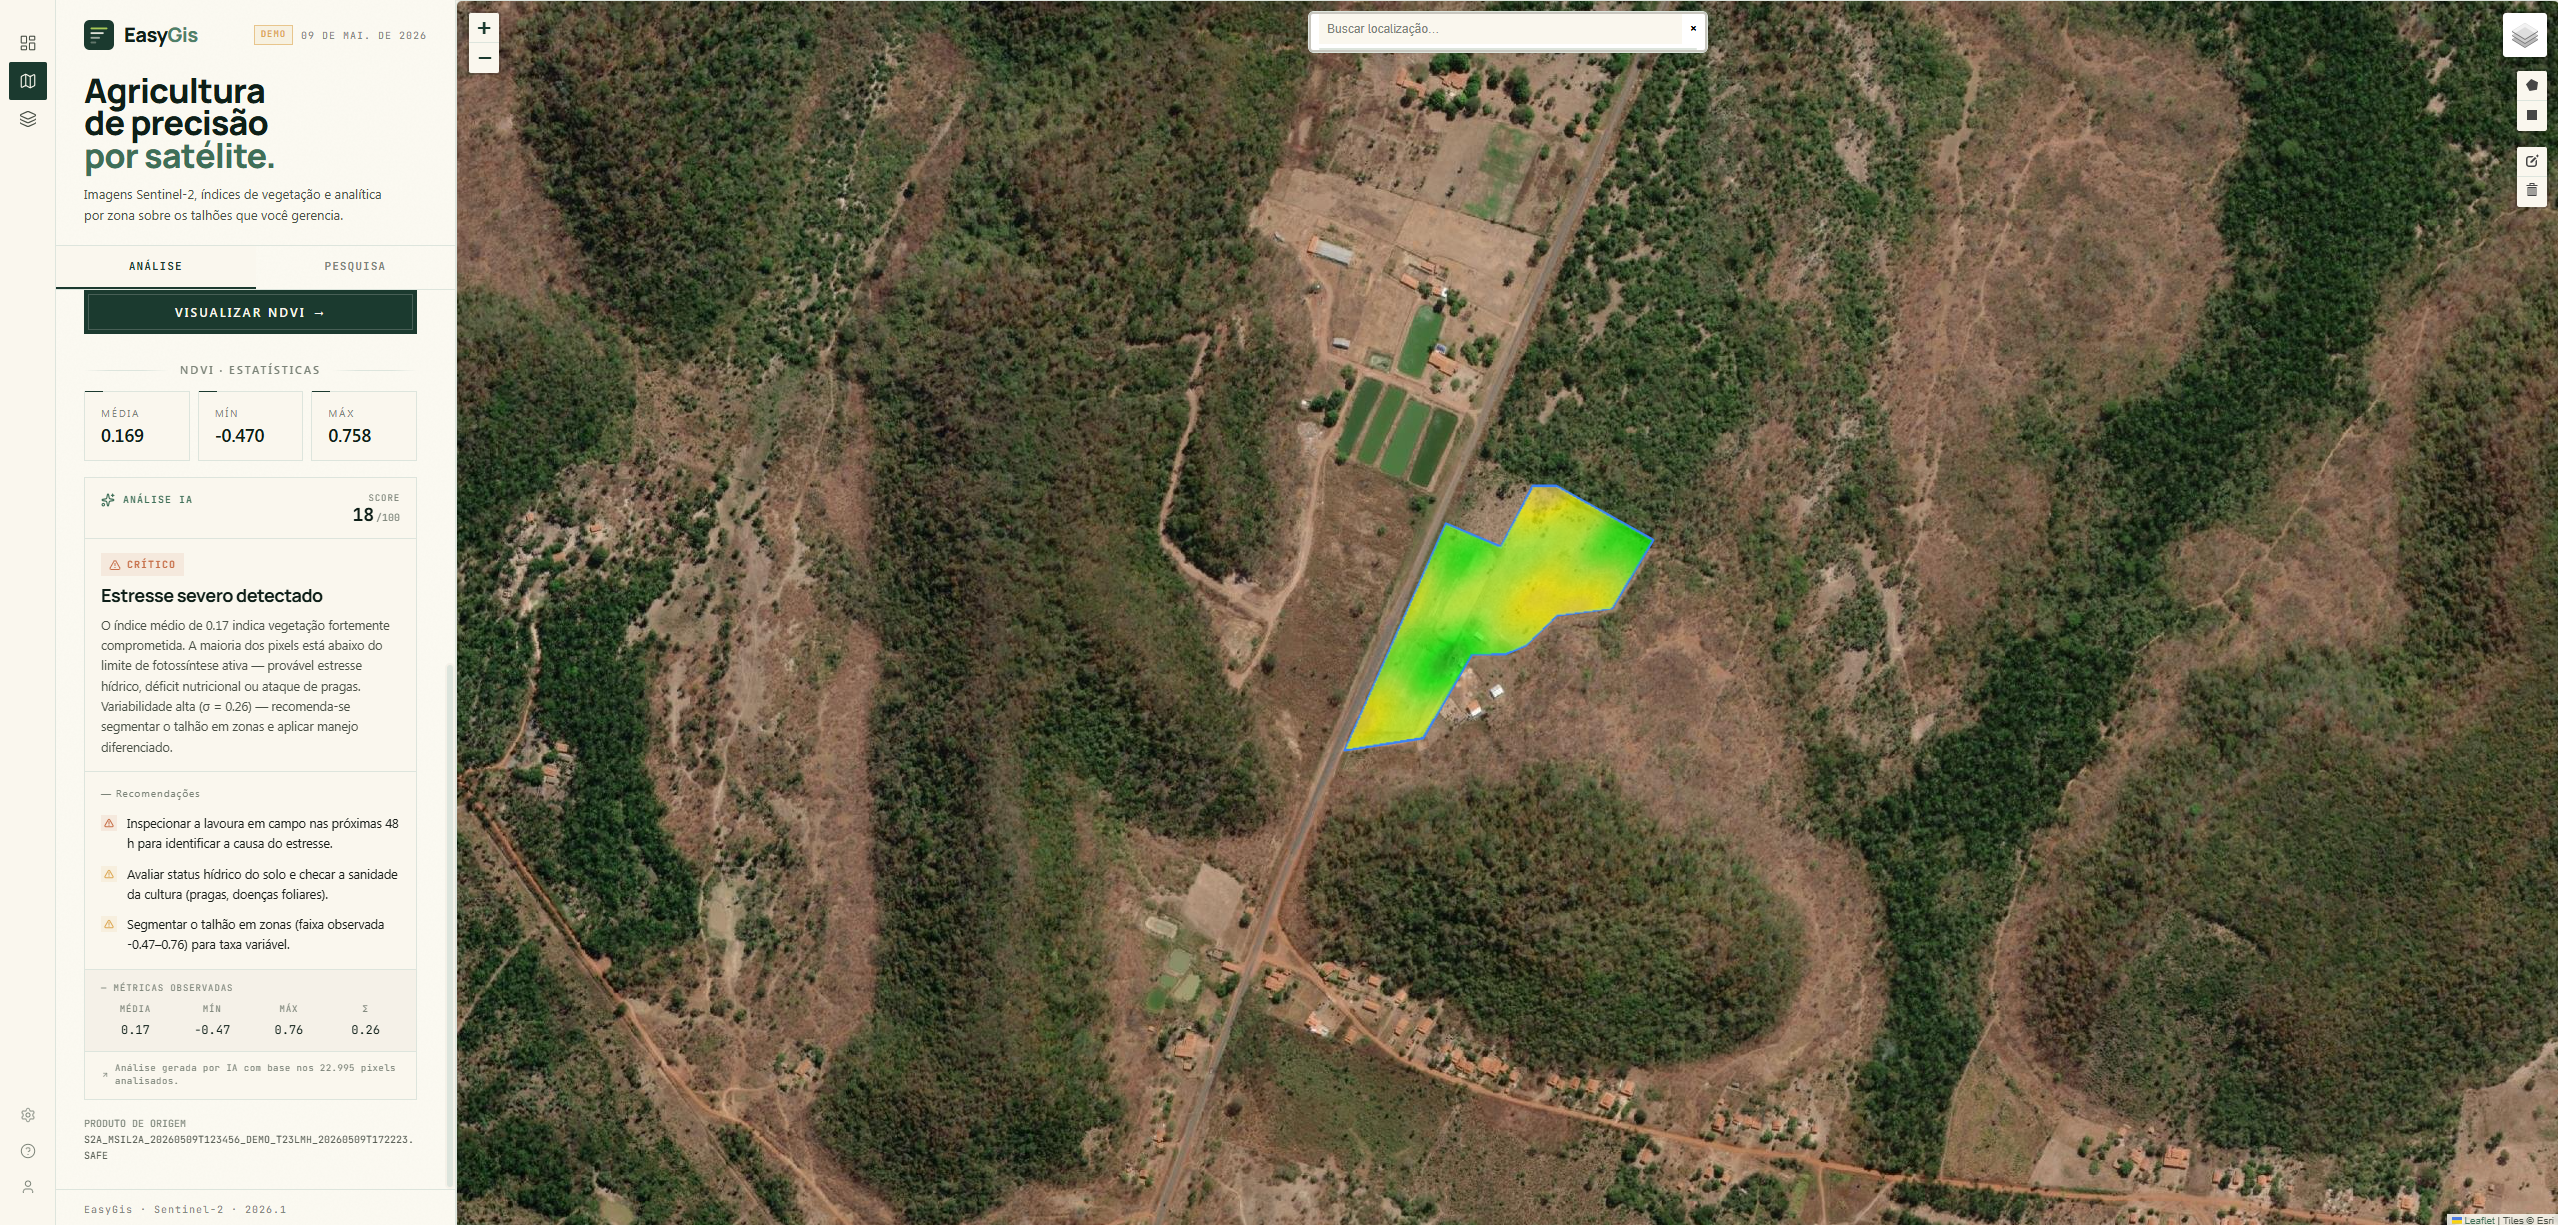
\includegraphics[width=\textwidth]{screenshots/MAN-03_ndvi-resultado}
\caption{Evidência visual de RF-05 (NDVI) + RF-10 (estatísticas) + RF-11 (histograma) --- saída da rota \texttt{POST /calculate-index} com \texttt{index\_type=NDVI} sobre o talhão \texttt{crop field 1}.}
\end{figure}

\begin{figure}[H]
\centering
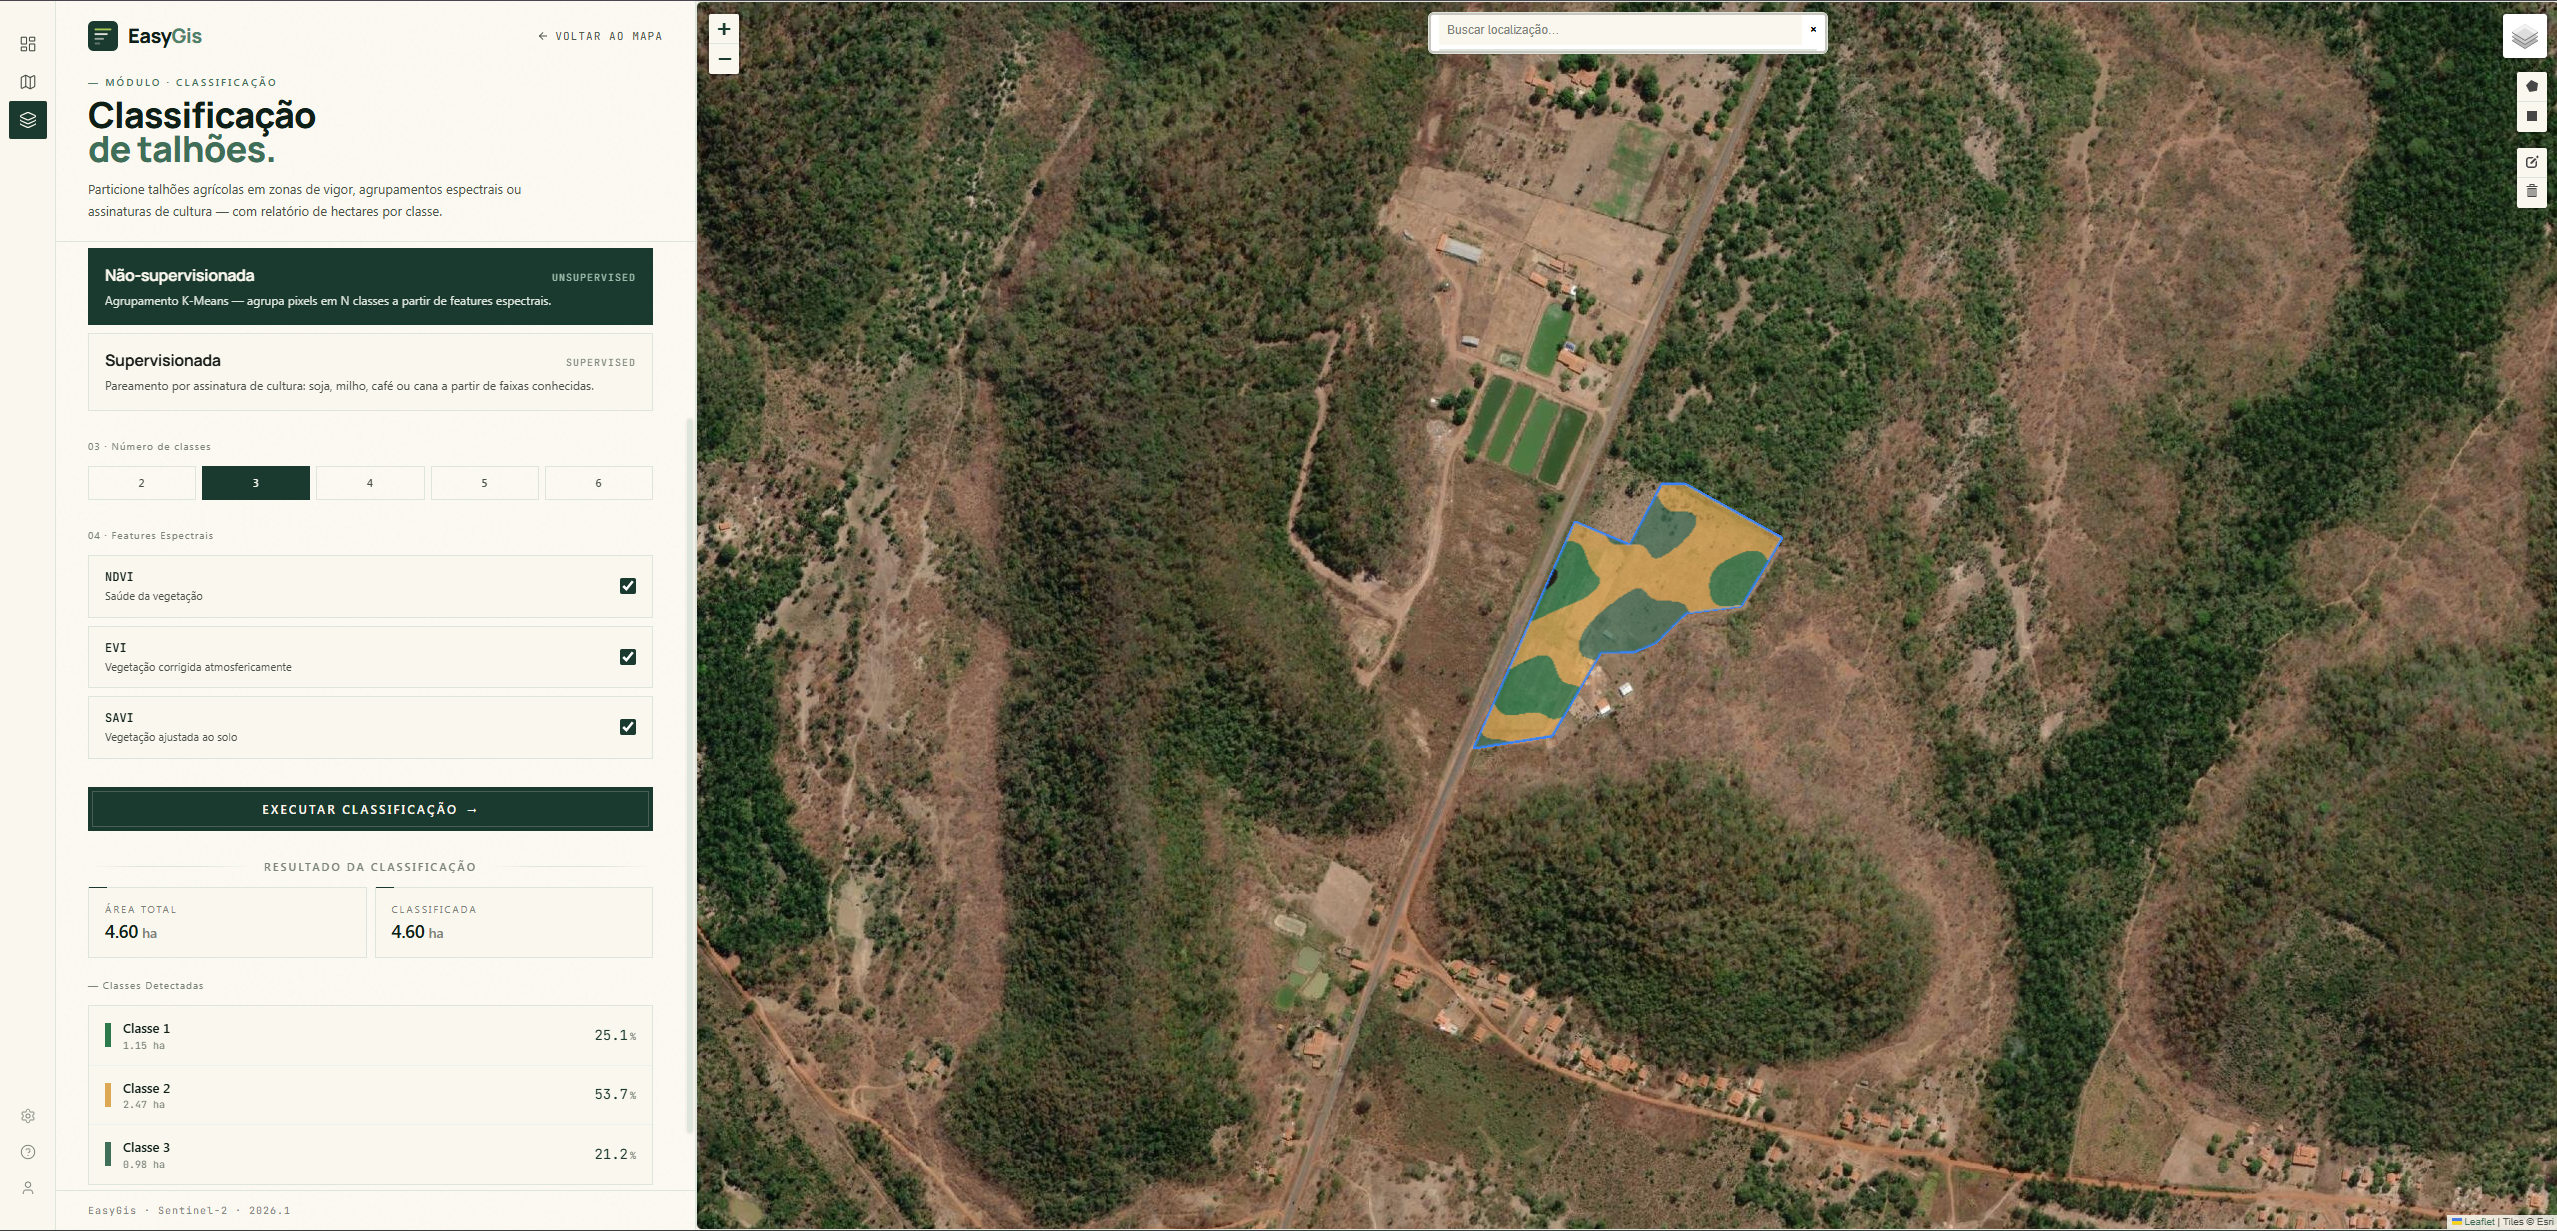
\includegraphics[width=\textwidth]{screenshots/MAN-07_classification}
\caption{Evidência visual da rota \texttt{POST /api/classification/classify} --- método K-Means com 3 classes, retornando porcentagem e área em hectares por classe.}
\end{figure}

% ══════════════════════════════════════════════════════════════
\section{Análise dos Resultados}
% ══════════════════════════════════════════════════════════════

\subsection{Pontos fortes}

\begin{enumerate}
  \item \textbf{Cobertura adequada da lógica de negócio.} Todas as funções puras de cálculo do \texttt{SentinelProcessor} (NDVI, EVI, estatísticas, histograma) estão cobertas, com casos felizes e de borda.
  \item \textbf{Validação Pydantic exercitada.} Os três caminhos de erro do endpoint principal (\texttt{/calculate-index}) --- body vazio, tipo errado, índice desconhecido --- produzem códigos HTTP corretos (422 / 400--500). Isso garante o RNF-04 (Confiabilidade --- erros claros).
  \item \textbf{Casos de borda explícitos.} Divisão por zero, arrays totalmente NaN, e conversão de tipo uint16 $\rightarrow$ float32 são testes que evitam regressões silenciosas se o código for refatorado.
  \item \textbf{Execução rápida.} A suite completa roda em $< 1$\,s (após cache de import), o que viabiliza inclusão em pipeline de CI futuro sem impacto perceptível.
  \item \textbf{Validação matemática.} O CT-01.3 verifica a fórmula com valores conhecidos analiticamente ($(8000-2000)/(8000+2000) = 0{,}6$), evitando bugs onde ``compila e roda mas calcula errado''.
\end{enumerate}

\subsection{Limitações conhecidas}

\renewcommand{\arraystretch}{1.4}
\begin{table}[H]
\centering
\small
\rowcolors{2}{tabrow}{white}
\begin{tabularx}{\textwidth}{@{}XXX@{}}
\toprule
\rowcolor{tabheader}\textcolor{white}{\textbf{Limitação}} & \textcolor{white}{\textbf{Justificativa}} & \textcolor{white}{\textbf{Mitigação}}\\
\midrule
Cobertura de \texttt{main.py} em 20\% & Endpoints de processamento exigem produto Sentinel-2 real ($\sim$1\,GB) que não cabe no repositório & Validação manual na demonstração ao vivo (Item 4 da P2)\\
Funções \texttt{read\_band} e \texttt{crop\_to\_geometry} não unitarizadas & Idem --- exigem JP2 real e granule structure do Sentinel-2 & Validação por demonstração end-to-end\\
Frontend (Next.js) não testado automaticamente & Escopo da P2 priorizou testes do backend (lógica de cálculo) & Validação manual via roteiro de demonstração\\
\bottomrule
\end{tabularx}
\end{table}

\subsection{Riscos residuais}

\begin{itemize}
  \item \textbf{Refatorações de I/O em \texttt{read\_band}} podem quebrar sem que a suite detecte. \textit{Mitigação:} incluir um teste de smoke com produto pequeno em uma futura iteração.
  \item \textbf{Mudanças no schema Pydantic} sem atualização do frontend podem causar erros 422 em produção. \textit{Mitigação:} TypeScript no cliente espelha o schema (DA-07), reduzindo risco.
\end{itemize}

% ══════════════════════════════════════════════════════════════
\section{Conclusão}
% ══════════════════════════════════════════════════════════════

A suíte de 54 testes valida com sucesso os requisitos funcionais críticos do MVP:

\begin{itemize}
  \item \textbf{RF-04, RF-05, RF-06, RF-10, RF-11, RF-20} --- todos cobertos.
  \item \textbf{RNF-04 (Confiabilidade), RNF-05 (Manutenibilidade)} --- exercitados estruturalmente.
\end{itemize}

\begin{successbox}
Não foram encontrados defeitos durante a execução. O sistema está apto à demonstração e entrega da P2.
\end{successbox}

% ══════════════════════════════════════════════════════════════
\section{Como Reproduzir}
% ══════════════════════════════════════════════════════════════

\begin{lstlisting}[style=shellstyle]
# Instalar dependencias (uma vez)
uv sync --group dev

# Rodar suite completa
uv run pytest tests/ -v

# Com cobertura
uv run pytest tests/ -v --cov=api --cov-report=term-missing

# Rodar um caso especifico (exemplo)
uv run pytest tests/test_sentinel_processor.py::TestNDVI::test_ndvi_formula_correctness -v
\end{lstlisting}

A suite é determinística (\texttt{np.random.default\_rng(seed=42)}), portanto os resultados são reprodutíveis em qualquer máquina com Python 3.12 e \texttt{uv} instalados.

\end{document}
